\clearpage

\section{Further studies for $\delta_{CP}$}
\label{subsec:deltaCP}

Further studies were performed in order to understand the results for $\delta_{CP}$  in Sec. \ref{app:fitter_performance}.
The residuals (fitted value - true input value) for $\delta_{CP}$ in figures \ref{fig:residuals_40_first}-\ref{fig:residuals_483_last} show that the 
fitter tends to return 0 or $\pm \pi$ irrespective of the true input value. This behaviour is due to the correlations between 
$\sin^{2}\theta_{13}$ and $\delta_{CP}$ as it will be explained in this section. 

To see how the correlation between $\sin^{2}\theta_{13}$ and $\delta_{CP}$ explains 
the distribution of residuals, the following test was performed:

\begin{enumerate}
\item{For one toy experiment with the same true input values as in Fig.\ref{fig:residuals_40_first} and no fluctuations, 
the true $\chi^{2}$ surface in ($\sin^{2}\theta_{13}$,$\delta_{CP}$) space 
(fixing $\sin^{2}\theta_{23}$ and $|\Delta m^{2}|$ to their input values) was built. The true $\chi^{2}$ surface can be found in Fig. \ref{fig:truechisqsurface}.
Notice that when zooming the true $\chi^{2}$ surface around a value of $\sin^{2}\theta_{13}$ (Fig. \ref{fig:truechisqsurface}, right plot) 
the difference in $\chi^{2}$ for different values of $\delta_{CP}$ is very small at current POT.}
\item{For a selected value of $\sin^{2}\theta_{13}$, the values of $\delta_{CP}$ in the true $\chi^{2}$ surface 
with a value of $\chi^{2}$ in a minimal band defined (with $\chi^{2}$ smaller than a certain value)
are found and a histogram is filled with them.} 
\item{Different values of $\sin^{2}\theta_{23}$ are selected following a Gaussian distribution around the 
true input value to reproduce the effect of the distribution of residuals for this parameter in Fig. \ref{fig:residuals_40_first}.} 
\end{enumerate}


\begin{figure}[htbp]
\begin{center}
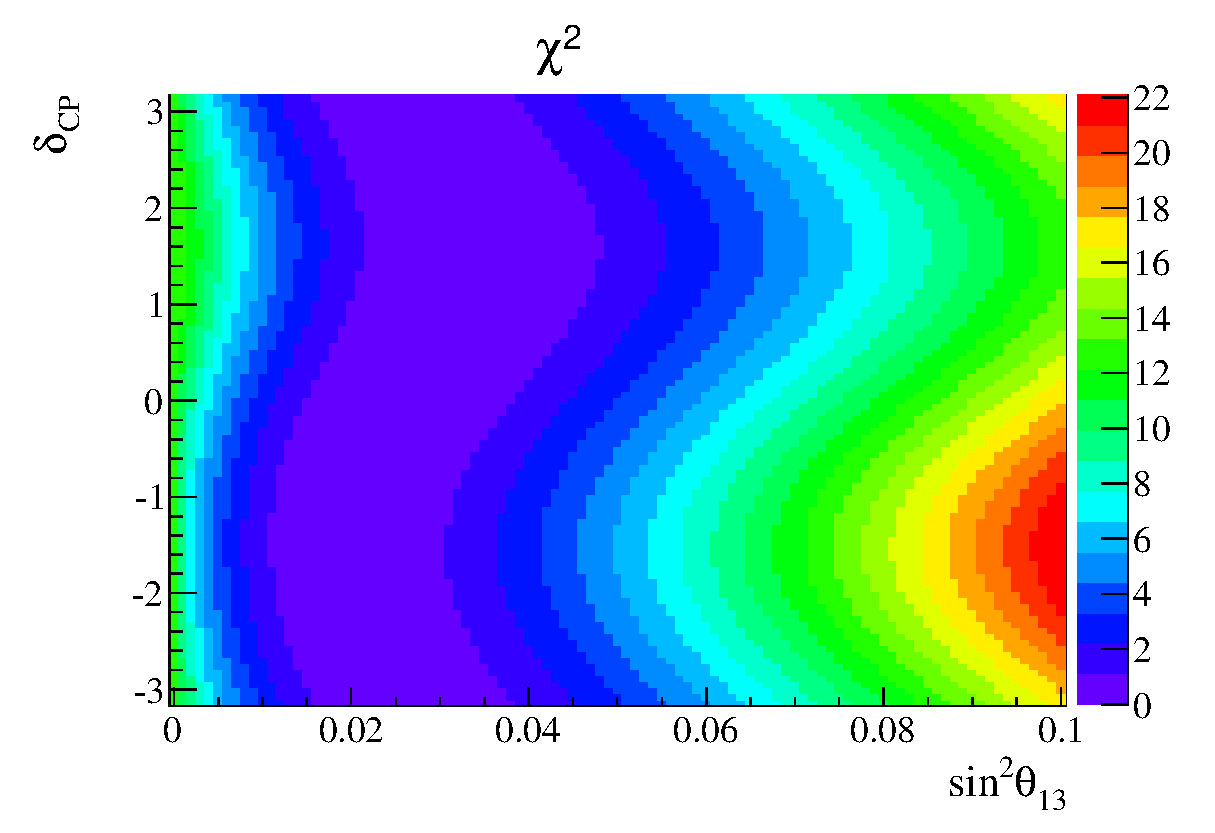
\includegraphics[width=0.5\textwidth]{images/appendix/deltacp/TrueChisqSurface.eps}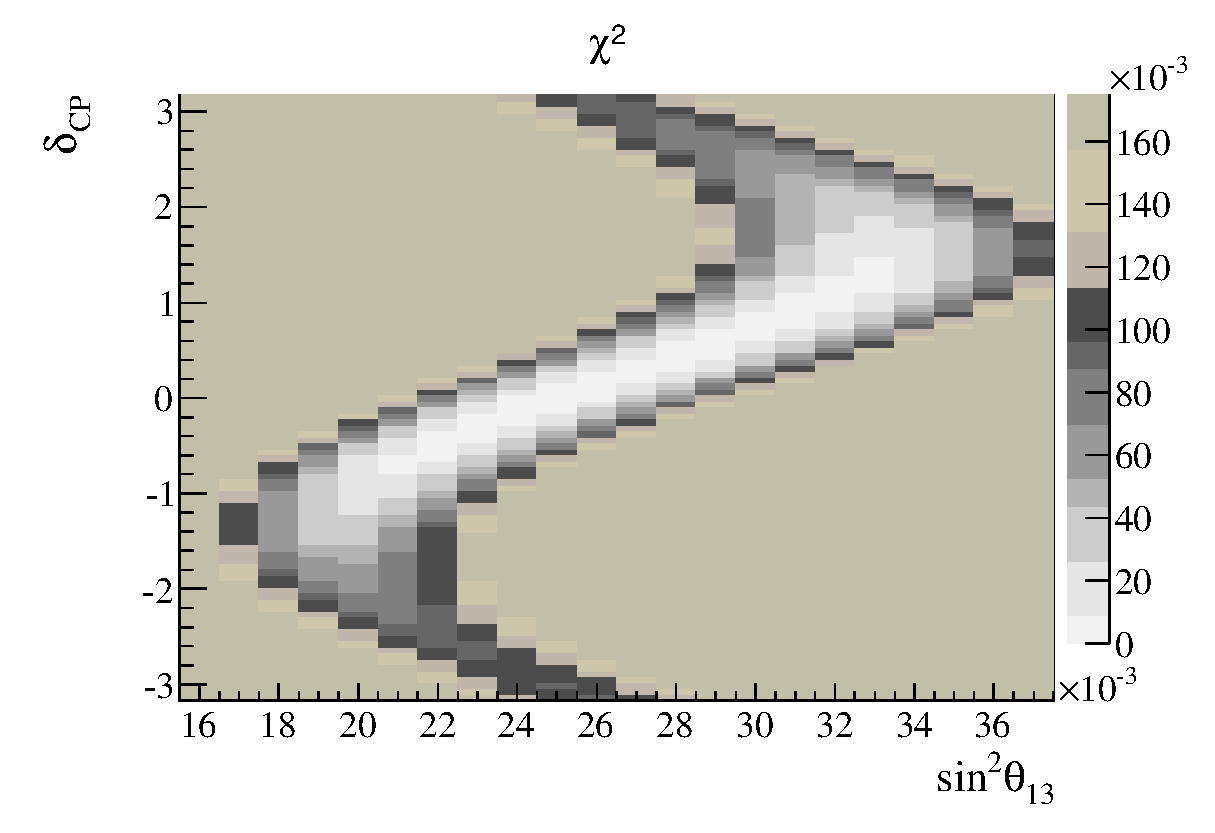
\includegraphics[width=0.5\textwidth]{images/appendix/deltacp/TrueChisqSurfaceZoom.eps}
\caption{True $\chi^{2}$ surface in ($\sin^{2}\theta_{13}$,$\delta_{CP}$) space for a toy experiment with 
true input values $\sin^{2}\theta_{23}= 0.5$, $|\Delta m^{2}| = 2.36\times10^{-3}(eV^{2}/c^{4})$, $\sin^{2}\theta_{13}=0.025$ and $\delta_{CP}$=0
and no fluctuations, fixing $\sin^{2}\theta_{23}$ and $|\Delta m^{2}|$ to their input values. Right, same true $\chi^{2}$ surface zoomed around true input value for $\sin^{2}\theta_{13}$.}
\label{fig:truechisqsurface}
\end{center}
\end{figure}


Figure \ref{fig:graphicexplanation} explains graphically the test made. Figure \ref{fig:graphicexplanation2} complements this explanation showing in left
top plot the density of points in the true $\chi^{2}$ minimal band.

\begin{figure}[htbp]
\begin{center}
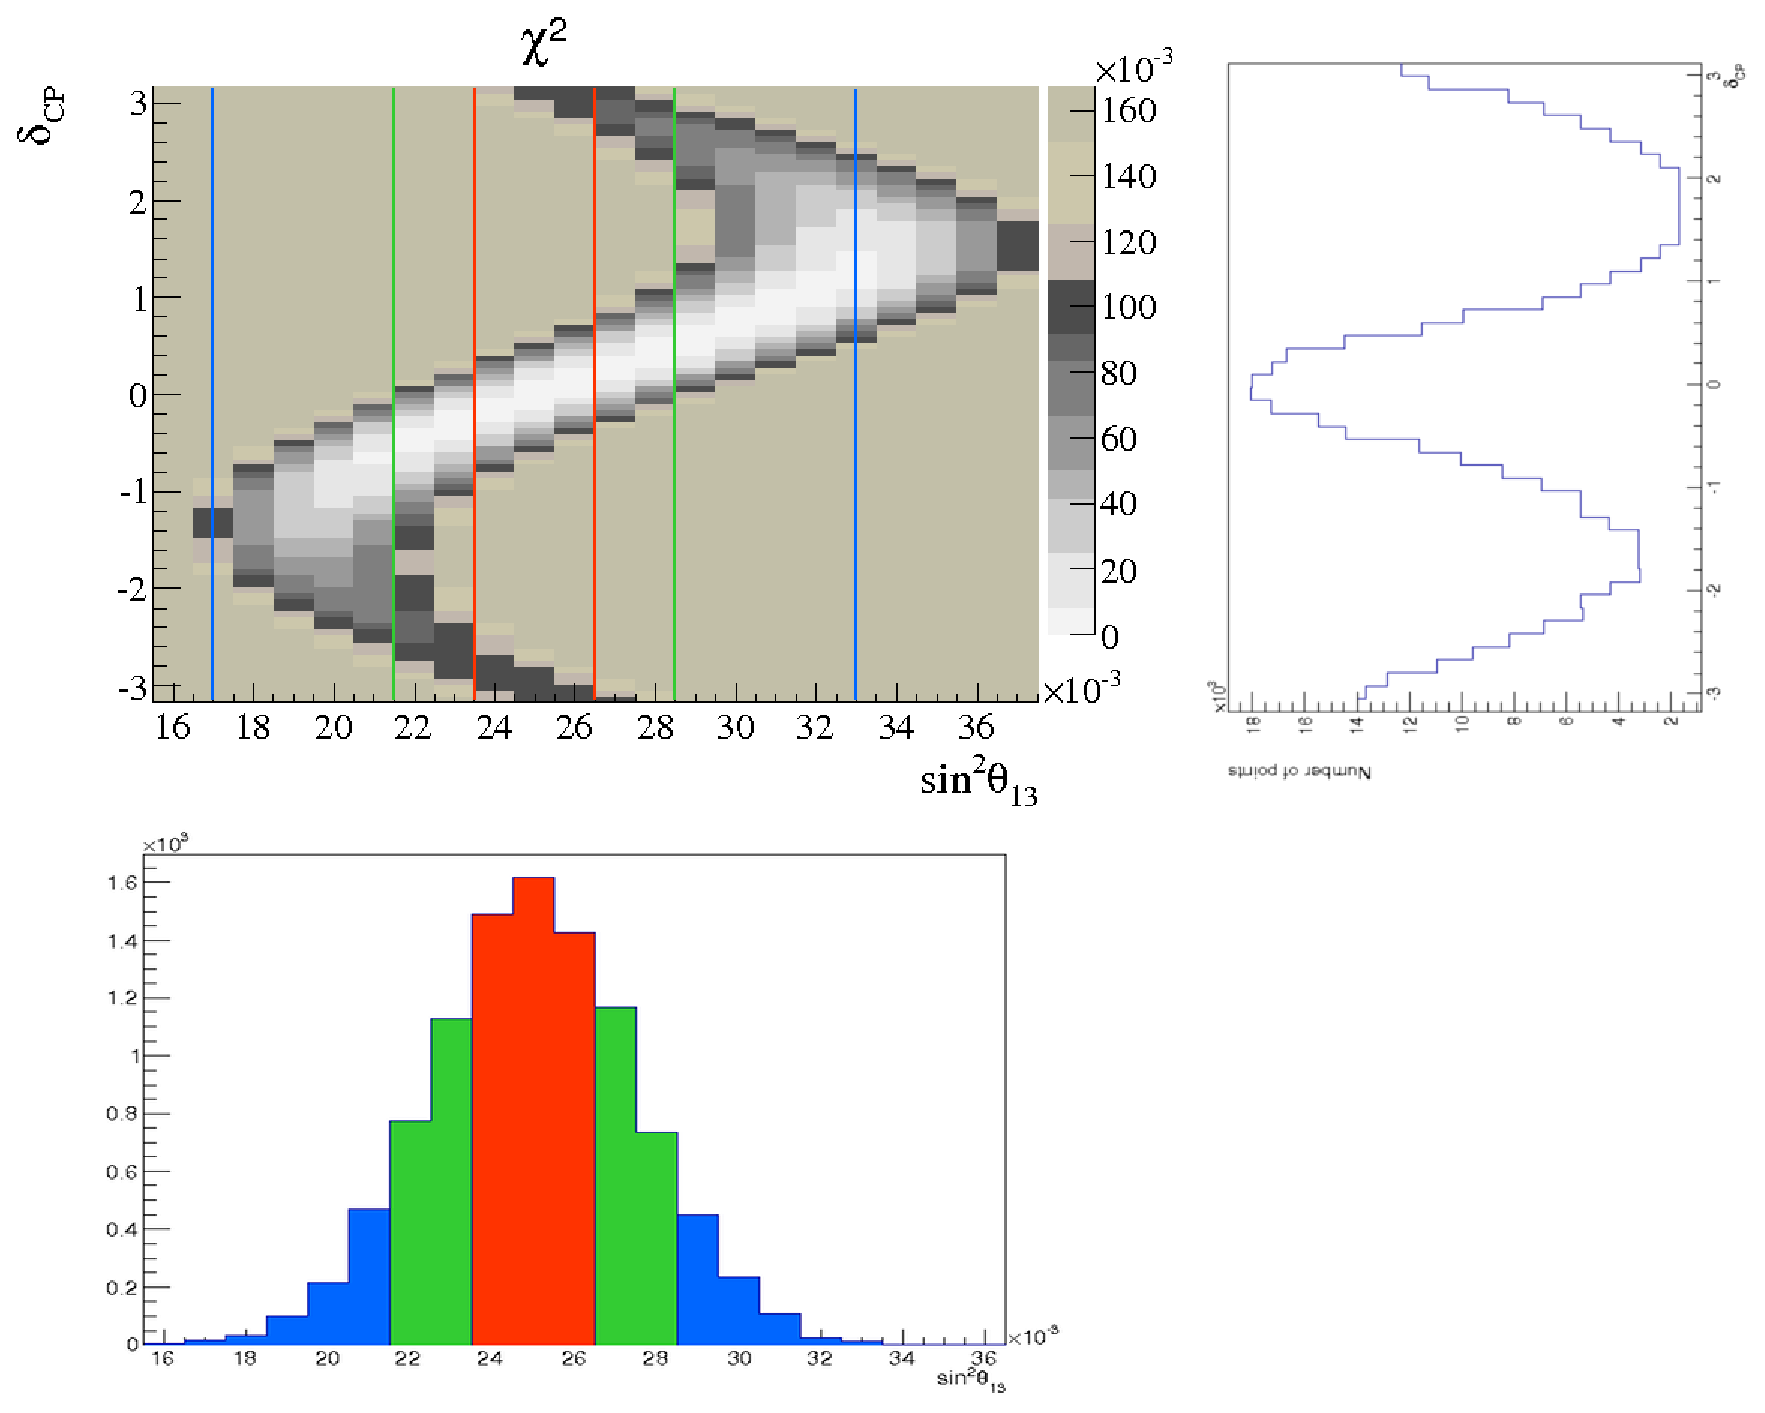
\includegraphics[width=0.7\textwidth]{images/appendix/deltacp/GraphicExplanationDeltaCPResiduals.eps}
\caption{Graphical explanation of the test made to understand the distribution of residuals for $\delta_{CP}$. 
For the Gaussian distribution of selected values of $\sin^{2}\theta_{13}$ (left bottom plot) the values of $\delta_{CP}$ 
in the true $\chi^{2}$ minimal band are found (left top plot) and a histogram is filled with them (right plot).}
\label{fig:graphicexplanation}
\end{center}
\end{figure}


\begin{figure}[htbp]
\begin{center}
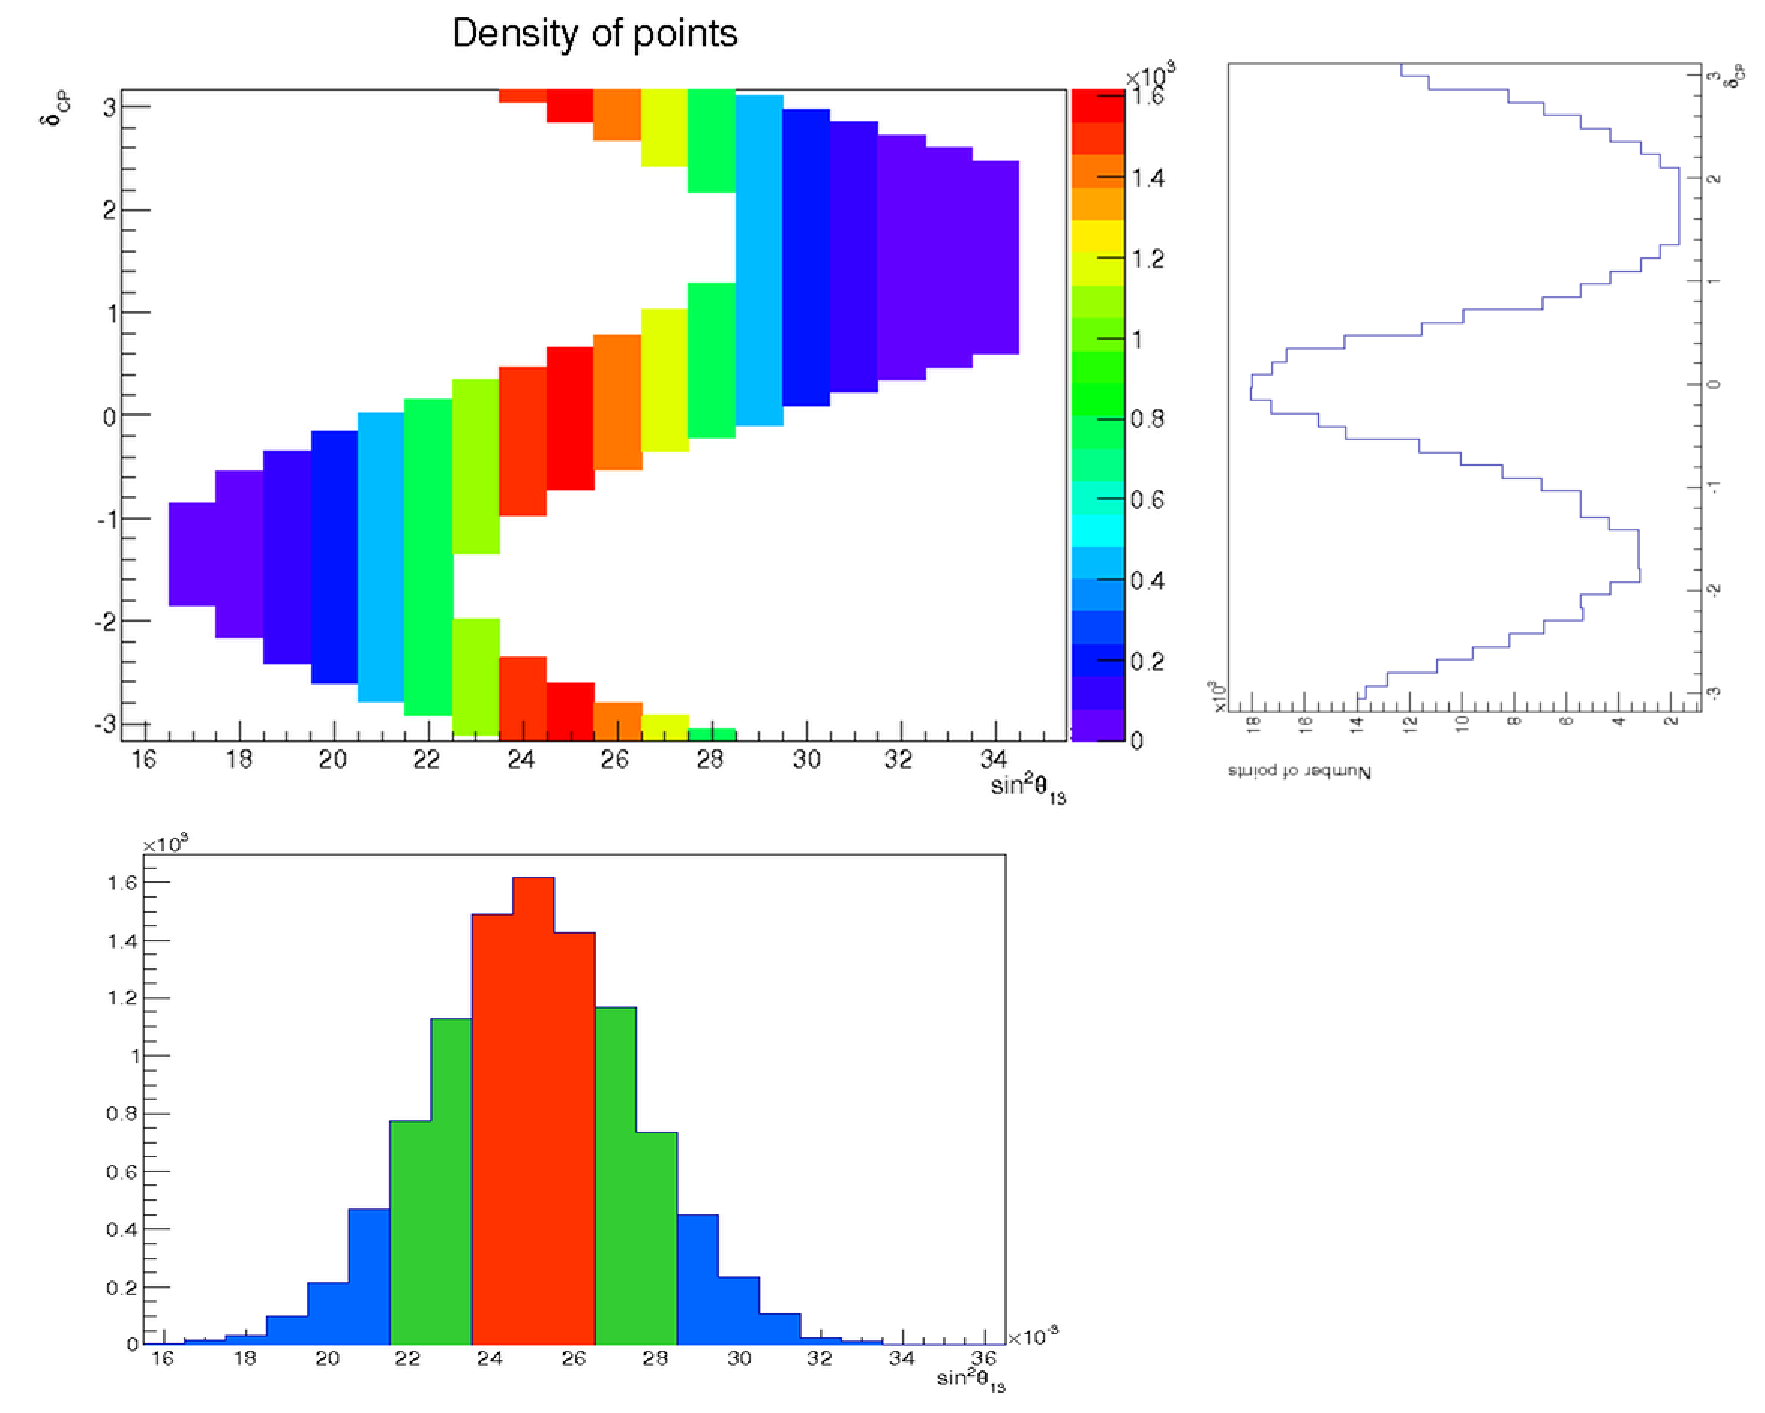
\includegraphics[width=0.7\textwidth]{images/appendix/deltacp/GraphicExplanationDeltaCPResiduals2.eps}
\caption{Graphical explanation of the test made to understand the distribution of residuals for $\delta_{CP}$. 
Same as in figure \ref{fig:graphicexplanation2} but replacing left top plot with the density of points in the true $\chi^{2}$ minimal band.}
\label{fig:graphicexplanation2}
\end{center}
\end{figure}


The result of the test (Fig. \ref{fig:resulttestdeltacp}, left plot) presents three peaks in the values of $\delta_{CP} = 0$ and $\delta_{CP} = \pm \pi$.
The fact that the $P_{\nu_{\mu}\rightarrow \nu_{e}}$ oscillation probability is almost identical for those values (see Fig. \ref{fig:oscprobdeltacp}) explains these three peaks
as well as the S-shape observed in the true $\chi^{2}$ surface in Fig. \ref{fig:truechisqsurface}. 

A more realistic result can be obtained if the test is repeated including the deviations in $\sin^{2}\theta_{23}$ and
$\sin^{2}\theta_{13}$ from Fig. \ref{fig:residuals_40_first}. 
This is done fixing $\sin^{2}\theta_{23}$ in the construction of the true $\chi^{2}$ surface to a value slightly different to the one used
to create the toy experiment and centering the Gaussian distribution of selected values of $\sin^{2}\theta_{13}$ slightly biased 
with respect to its true input value.
In this case the central peak is not centered at 0 but biased as can be observed in Fig. \ref{fig:resulttestdeltacp}, right plot, 
in good agreement with the distribution of residuals for $\delta_{CP}$ in Fig. \ref{fig:residuals_40_first}.

\begin{figure}[htbp]
\begin{center}
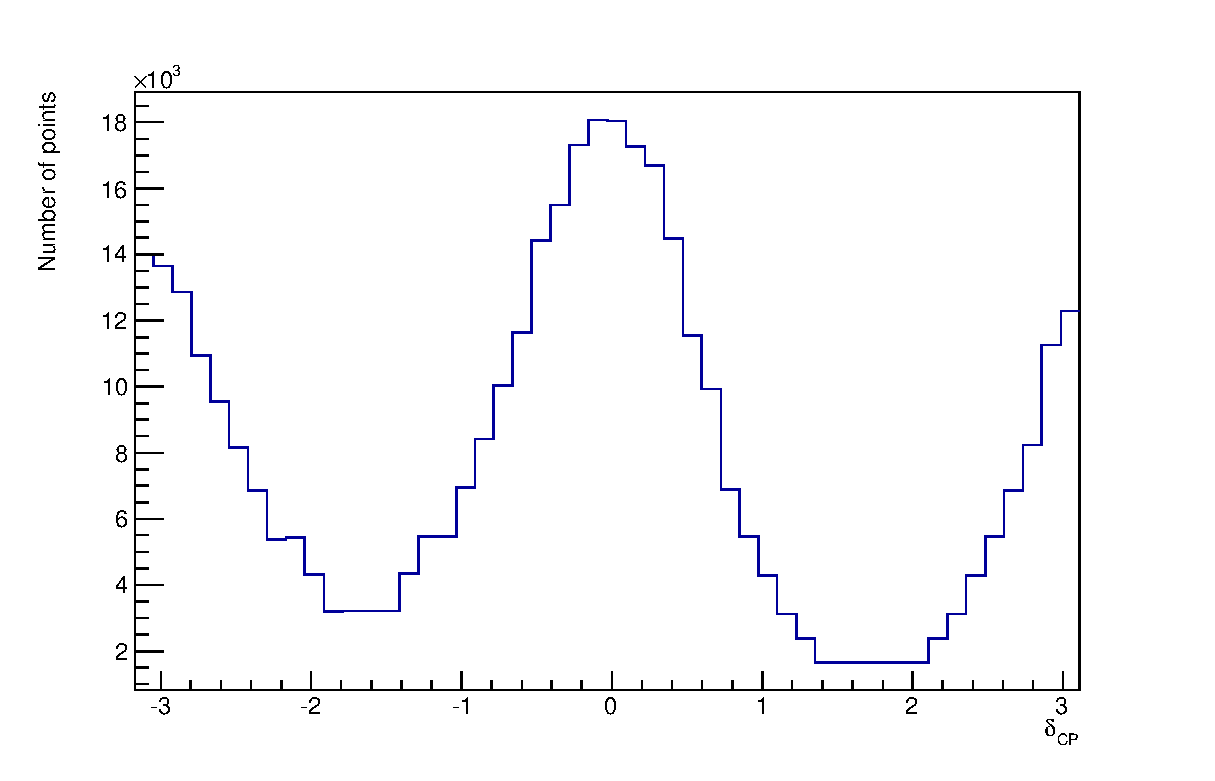
\includegraphics[width=0.5\textwidth]{images/appendix/deltacp/DeltaCPDistribution.eps}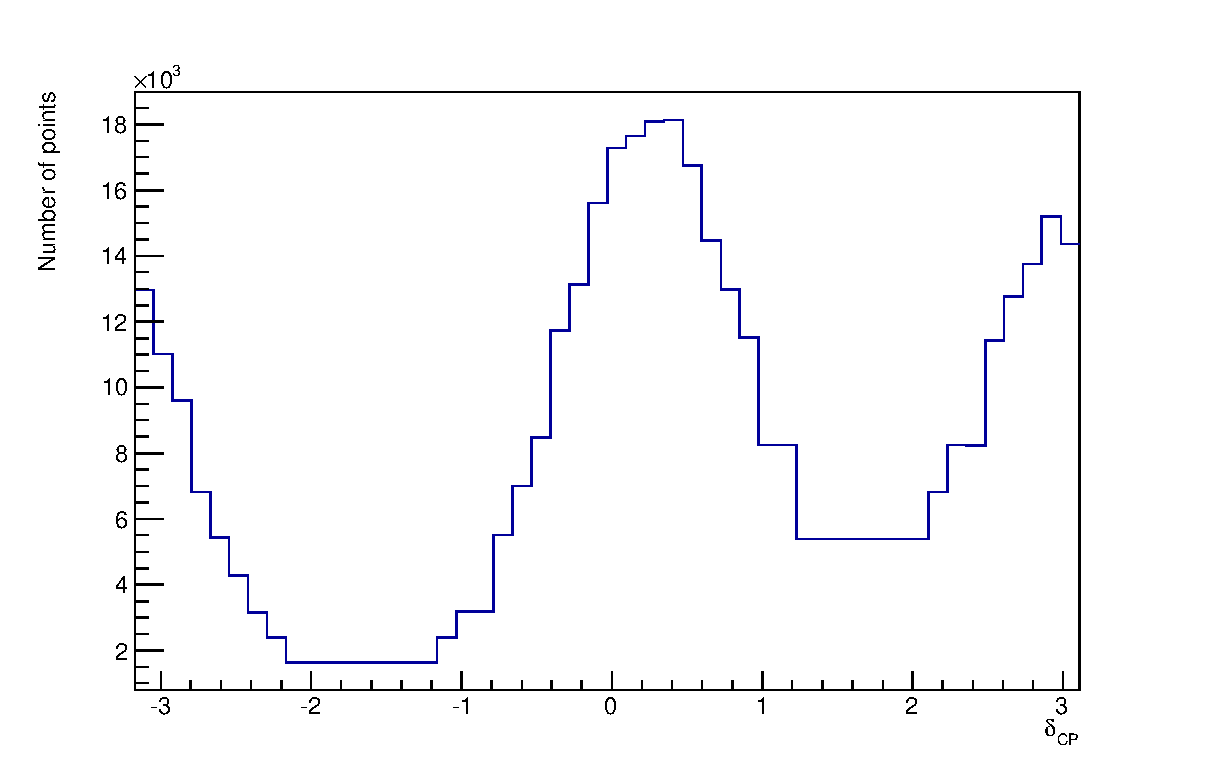
\includegraphics[width=0.5\textwidth]{images/appendix/deltacp/DeltaCPDistributionBiased.eps}
\caption{Result of the test explained in figure \ref{fig:graphicexplanation}, i.e. the distribution of selected points vs $\delta_{CP}$. 
On the left, perfect case. On the right, realistic case including the deviations in $\sin^{2}\theta_{23}$ and
$\sin^{2}\theta_{13}$ from Fig. \ref{fig:residuals_40_first}.}
\label{fig:resulttestdeltacp}
\end{center}
\end{figure}

\begin{figure}[htbp]
\begin{center}
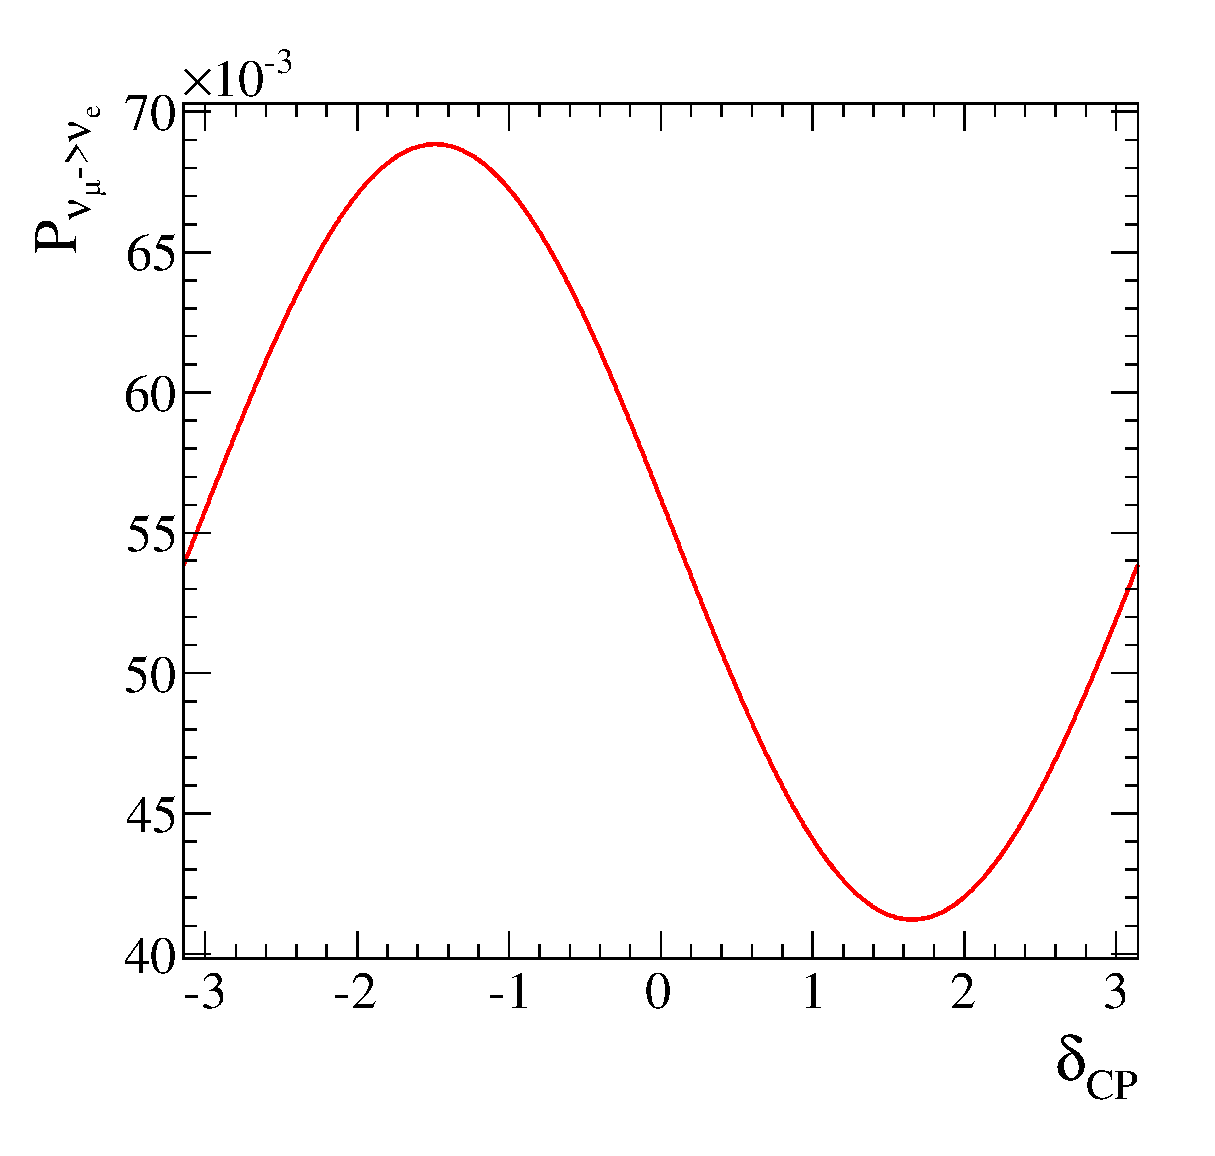
\includegraphics[width=0.5\textwidth]{images/appendix/deltacp/OscProbDeltaCP.eps}
\caption{ $P_{\nu_{\mu}\rightarrow \nu_{e}}$ oscillation probability vs $\delta_{CP}$
with values $\sin^{2}\theta_{23}= 0.5$, $|\Delta m^{2}| = 2.36\times10^{-3}(eV^{2}/c^{4})$ and $\sin^{2}\theta_{13}=0.025$.}
\label{fig:oscprobdeltacp}
\end{center}
\end{figure}

Now the test was performed again using as true input values  $\delta_{CP} = \pm \pi/2$. Figures \ref{fig:truechisqsurfacehalfpi} and \ref{fig:truechisqsurfacemhalfpi}
show the true $\chi^{2}$ surface in ($\sin^{2}\theta_{13}$,$\delta_{CP}$) space for a toy experiment without fluctuations with
true input value $\delta_{CP} =  \pi/2$  and $\delta_{CP} = -\pi/2$ respectively and a zoom around the true input value for $\sin^{2}\theta_{13}$. The rest of input values are the same as 
for Fig. \ref{fig:truechisqsurface}. From the zoom of the true $\chi^{2}$ surface (right plots in \ref{fig:truechisqsurfacehalfpi} and \ref{fig:truechisqsurfacemhalfpi}) it is clear that 
selecting values of $\sin^{2}\theta_{13}$ around its true input value is only going to intersect with the minimum band in one area, giving then a single peak 
in the distribution for $\delta_{CP}$.
The results of the test for these two toy experiments are shown in Fig. \ref{fig:resulttestdeltacppmhalfpi}
($\delta_{CP} =  \pi/2$ left plot, $\delta_{CP} =  -\pi/2$ right plot). Those results do not show three peaks as the test for $\delta_{CP} = 0$
but a single peak around the true input value, because no other values of $\delta_{CP}$ give the same value of $P_{\nu_{\mu}\rightarrow \nu_{e}}$ 
 as that for either $\delta_{CP} =  \pi/2$ or $\delta_{CP} =  -\pi/2$. 
 
 
However, to reproduce the results observed in Figs. \ref{fig:residuals_40_point5} and \ref{fig:residuals_40_point6}
is necessary to include the biases in $\sin^{2}\theta_{23}$ and $\sin^{2}\theta_{13}$ which are much more important now. 
The result is presented in Fig. \ref{fig:resulttestdeltacppmhalfpibiased}.
Notice that Figs.\ref{fig:residuals_40_point5} and \ref{fig:residuals_40_point6} show the distribution of residuals (bestfit - input value)
and the result of this test in Fig.\ref{fig:resulttestdeltacppmhalfpibiased} shows a distribution comparable to bestfit values (not (bestfit - input value) ).

 
 \begin{figure}[htbp]
\begin{center}
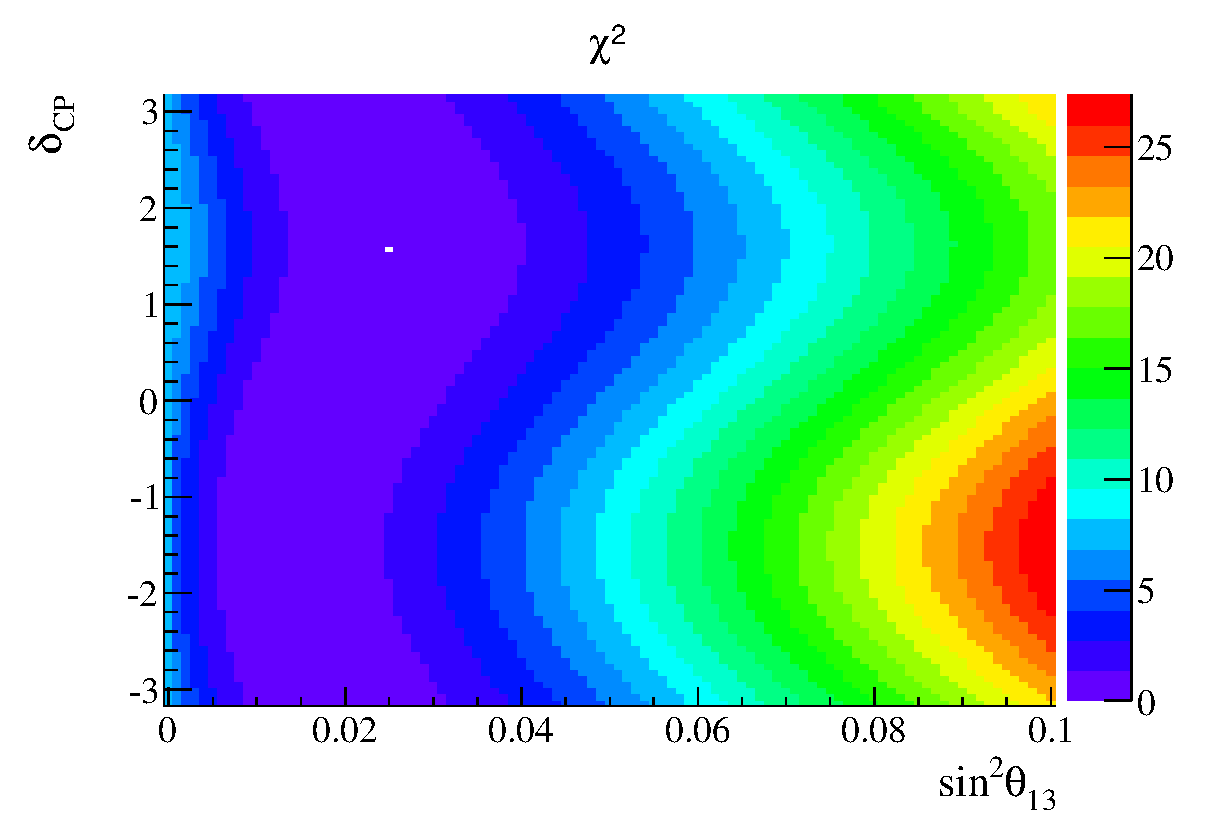
\includegraphics[width=0.5\textwidth]{images/appendix/deltacp/TrueChisqSurfaceHalfPi.eps}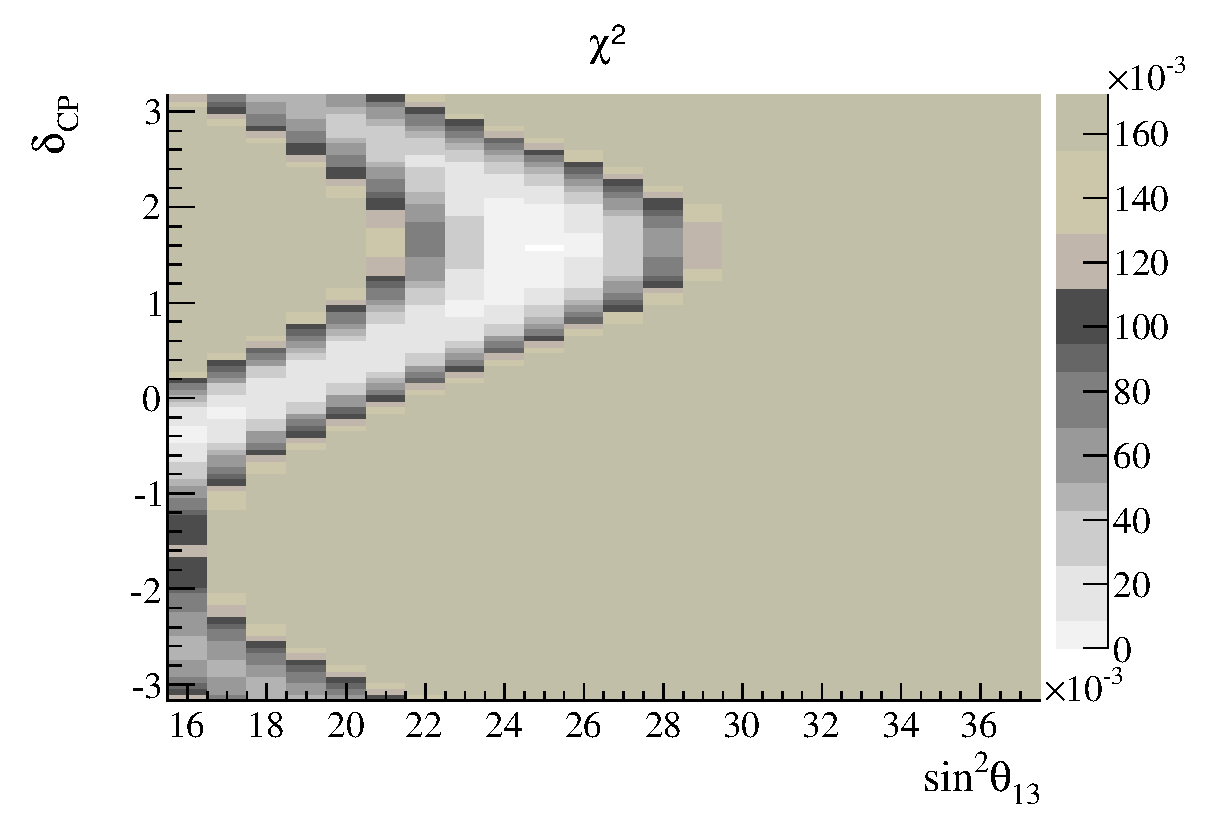
\includegraphics[width=0.5\textwidth]{images/appendix/deltacp/ChisqSurfaceZoomHalfPi.eps}
\caption{True $\chi^{2}$ surface in $\sin^{2}\theta_{13}$,$\delta_{CP}$) space for a toy experiment without fluctuations and with 
true input values $\sin^{2}\theta_{23}= 0.5$, $|\Delta m^{2}| = 2.36\times10^{-3}(eV^{2}/c^{4})$, $\sin^{2}\theta_{13}=0.025$ and $\delta_{CP} =\pi/2$,
 fixing $\sin^{2}\theta_{23}$ and $|\Delta m^{2}|$ to their input values. Right, same true $\chi^{2}$ surface zoomed around true input value for $\sin^{2}\theta_{13}$.}
\label{fig:truechisqsurfacehalfpi}
\end{center}
\end{figure}


 \begin{figure}[htbp]
\begin{center}
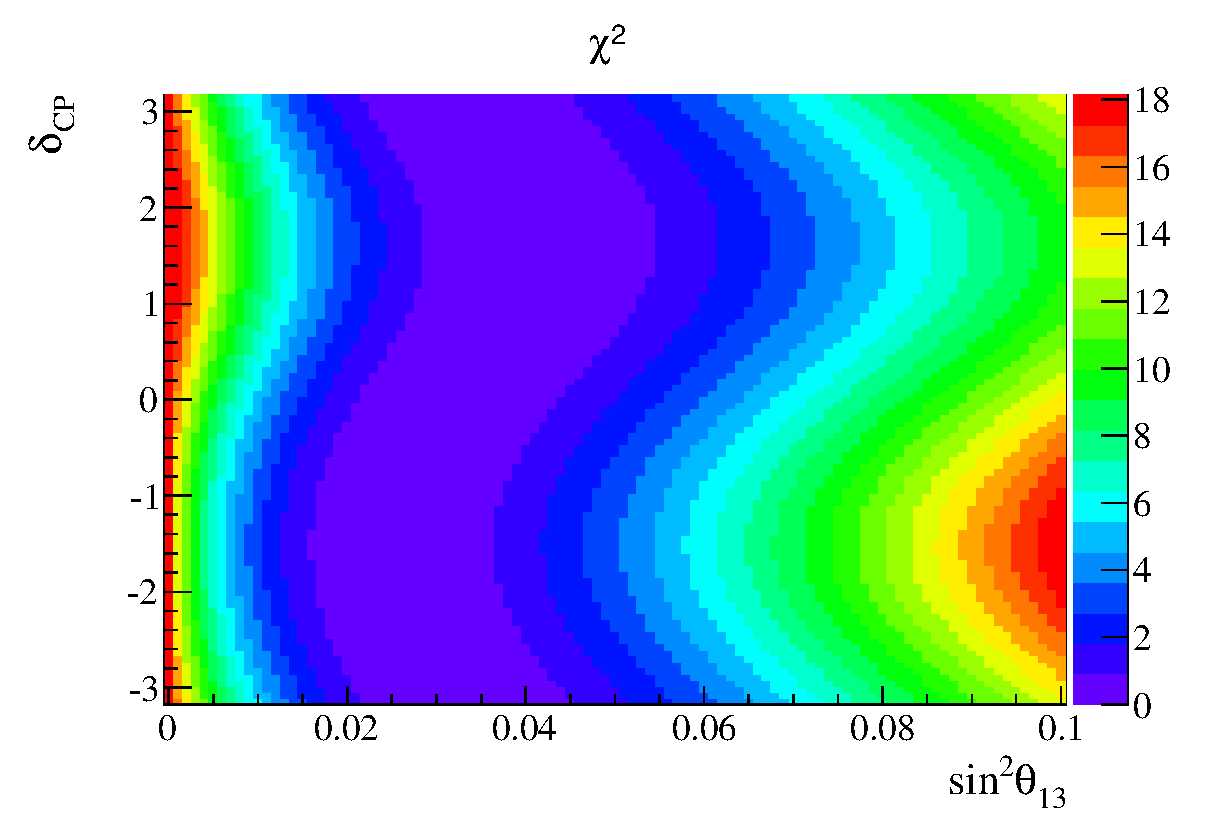
\includegraphics[width=0.5\textwidth]{images/appendix/deltacp/TrueChisqSurfaceMinusHalfPi.eps}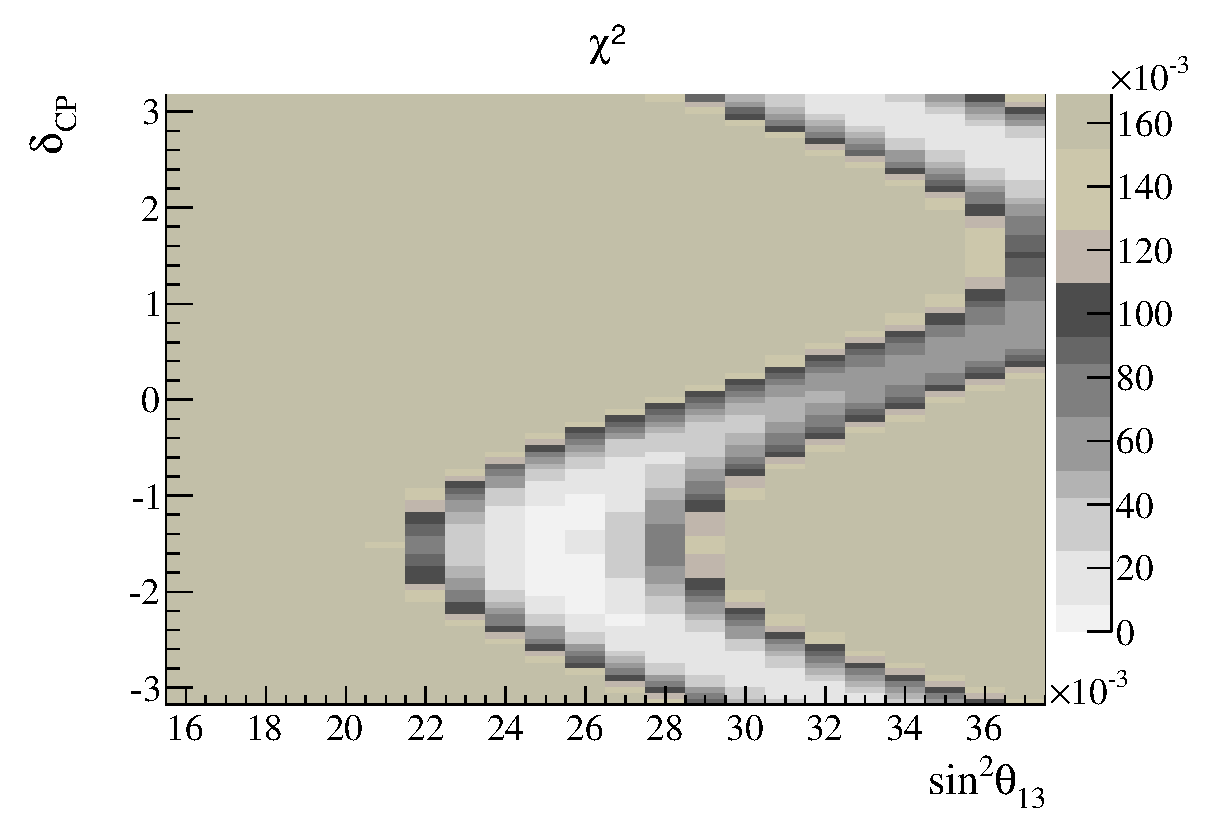
\includegraphics[width=0.5\textwidth]{images/appendix/deltacp/ChisqSurfaceZoomMHalfPi.eps}
\caption{True $\chi^{2}$ surface in $\sin^{2}\theta_{13}$,$\delta_{CP}$) space for a toy experiment without fluctuations and with 
true input values $\sin^{2}\theta_{23}= 0.5$, $|\Delta m^{2}| = 2.36\times10^{-3}(eV^{2}/c^{4})$, $\sin^{2}\theta_{13}=0.025$ and $\delta_{CP} =-\pi/2$,
 fixing $\sin^{2}\theta_{23}$ and $|\Delta m^{2}|$ to their input values. Right, same true $\chi^{2}$ surface zoomed around true input value for $\sin^{2}\theta_{13}$.}
\label{fig:truechisqsurfacemhalfpi}
\end{center}
\end{figure}
 
 
 \begin{figure}[htbp]
\begin{center}
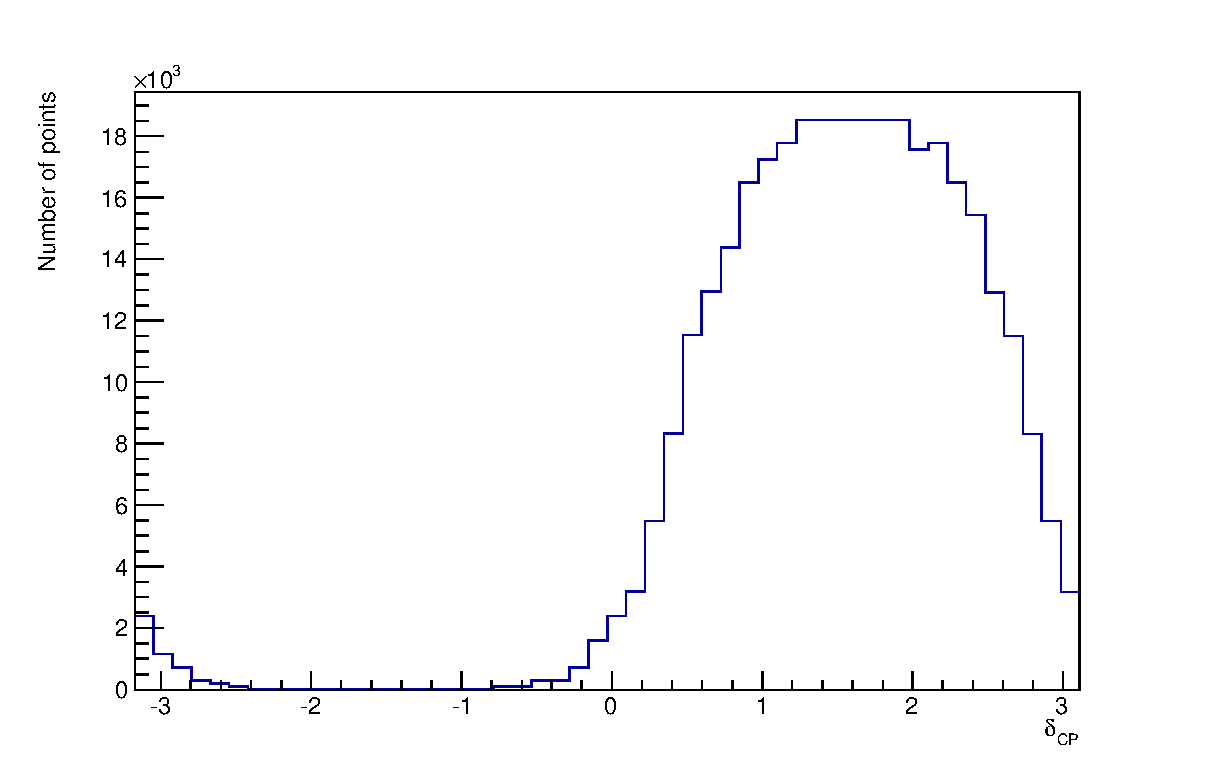
\includegraphics[width=0.5\textwidth]{images/appendix/deltacp/DeltaCPDistributionHalfPi.eps}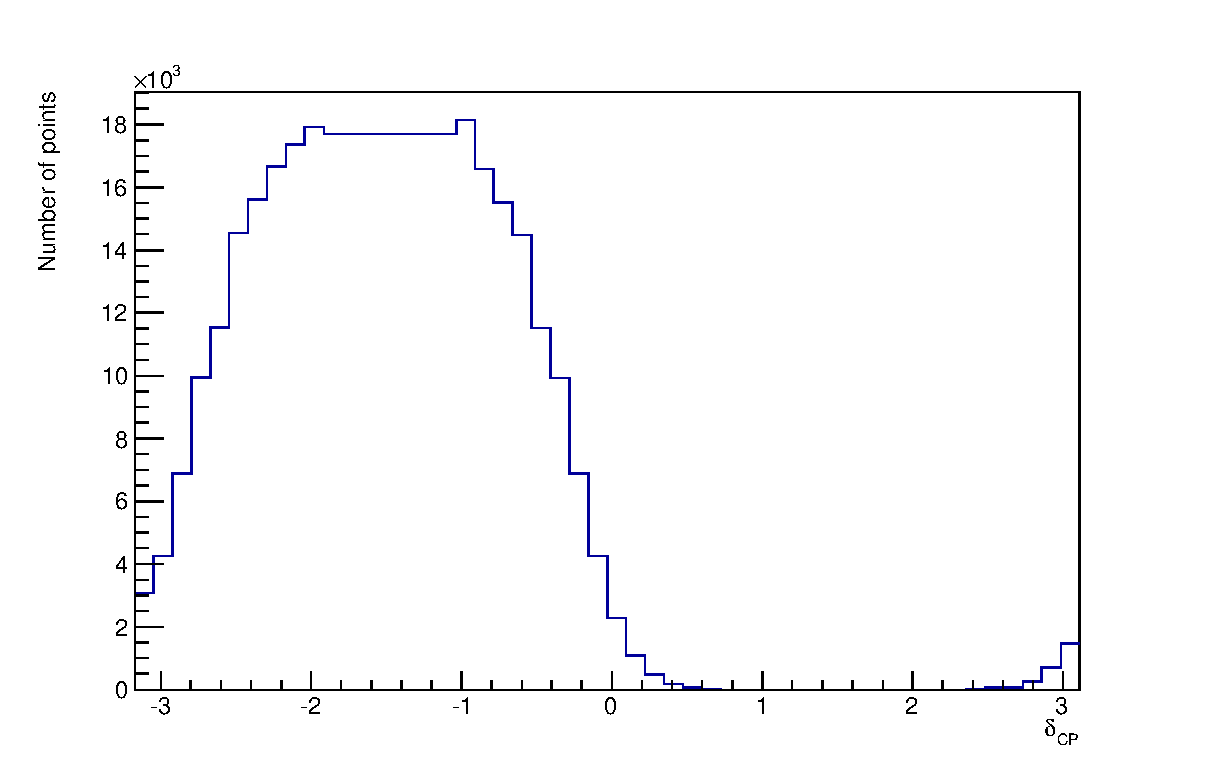
\includegraphics[width=0.5\textwidth]{images/appendix/deltacp/DeltaCPDistributionMinusHalfPi.eps}
\caption{Result of the test explained in figure \ref{fig:graphicexplanation}, i.e. the distribution of selected points vs $\delta_{CP}$. 
Left plot is for  $\delta_{CP} =  \pi/2$ and right plot is for $\delta_{CP} =  -\pi/2$.}
\label{fig:resulttestdeltacppmhalfpi}
\end{center}
\end{figure}
 
 
 The same test was repeated for $\delta_{CP} = \pm \pi/2$ including the biases in $\sin^{2}\theta_{23}$ and $\sin^{2}\theta_{13}$ from Figs.\ref{fig:residuals_40_point5} and \ref{fig:residuals_40_point6}.
 Notice that the bias in $\sin^{2}\theta_{13}$ is much larger than in the case of $\delta_{CP} = 0$ and with opposite senses 
 (mean in $\sin^{2}\theta_{13} \approx -0.005$ for $\delta_{CP} = \pi/2$ and  mean in $\sin^{2}\theta_{13} \approx 0.006$ for $\delta_{CP} = -\pi/2$, 
 while mean in $\sin^{2}\theta_{13} \approx 0.0007$ for $\delta_{CP} = 0$).
 The result of this new test is shown in Fig. \ref{fig:resulttestdeltacppmhalfpibiased}. As expected, even for those true input values of $\delta_{CP} =\pm \pi/2$
the distribution vs $\delta_{CP} $ presents three peaks at $\delta_{CP} =  0$ and $\delta_{CP} = \pm \pi$ when including the corresponding biases in 
$\sin^{2}\theta_{23}$ and $\sin^{2}\theta_{13}$.


 \begin{figure}[htbp]
\begin{center}
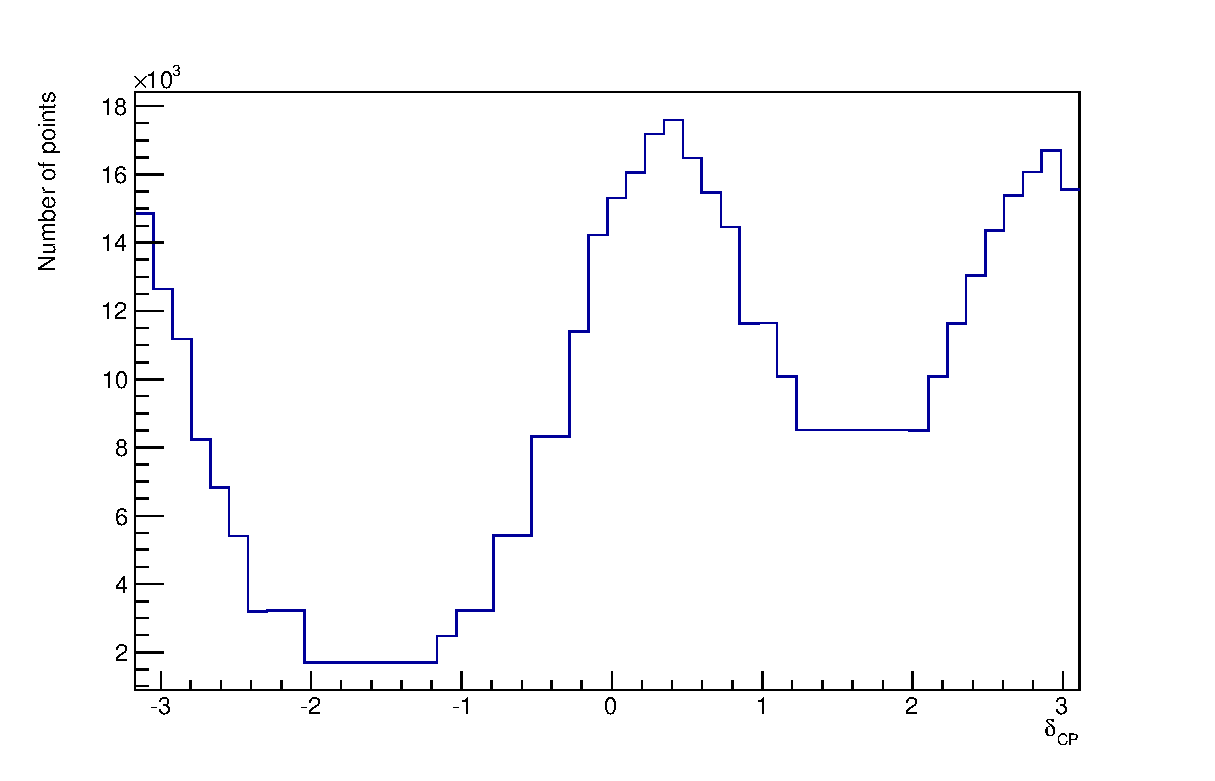
\includegraphics[width=0.5\textwidth]{images/appendix/deltacp/DeltaCPDistributionHalfPiBiased.eps}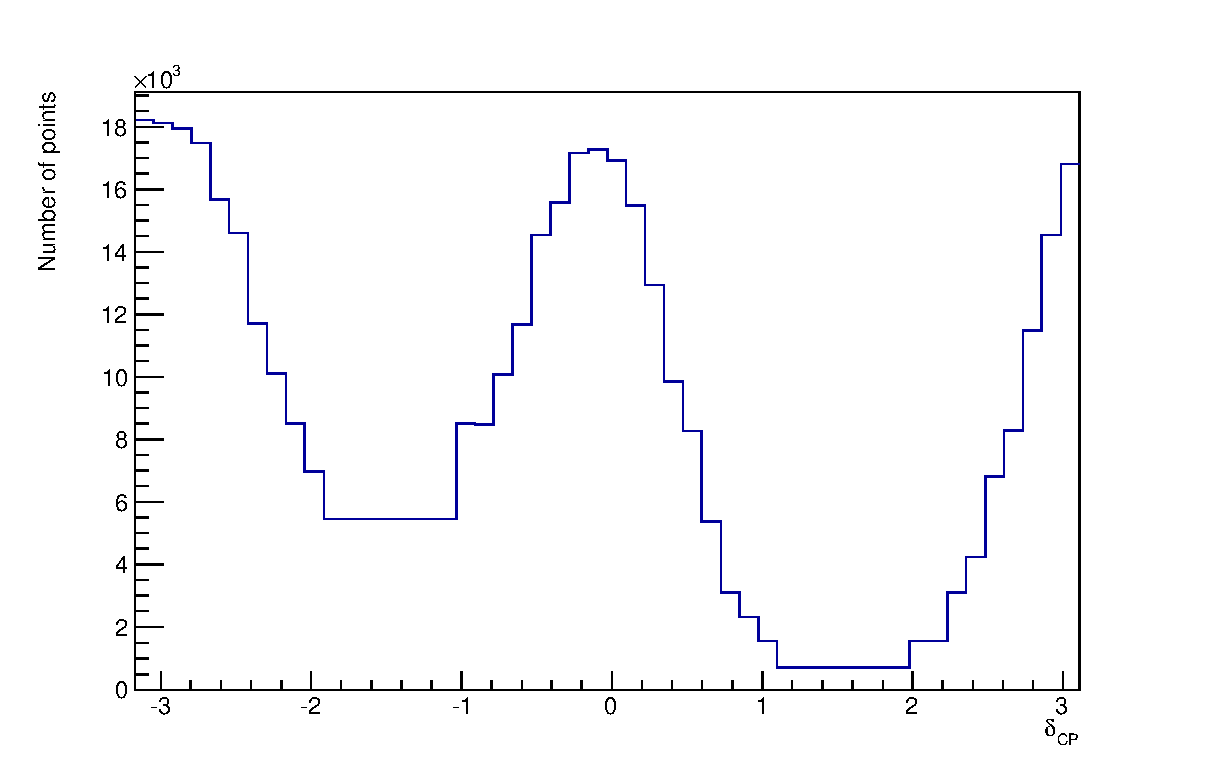
\includegraphics[width=0.5\textwidth]{images/appendix/deltacp/DeltaCPDistributionMinusHalfPiBiased.eps}
\caption{Result of the test explained in figure \ref{fig:graphicexplanation}, i.e. the distribution of selected points vs $\delta_{CP}$
when including the corresponding biases in $\sin^{2}\theta_{23}$ and $\sin^{2}\theta_{13}$ from  Figs. \ref{fig:residuals_40_point5} and \ref{fig:residuals_40_point6}.
Left plot is for  $\delta_{CP} =  \pi/2$ and right plot is for $\delta_{CP} =  -\pi/2$.}
\label{fig:resulttestdeltacppmhalfpibiased}
\end{center}
\end{figure}
 
 
An attempt was made to improve the sensitivity to $\delta_{CP}$ by constraining the fitted values of the other oscillation parameters. It was found that 
the sensitivity was improved if $\sin^{2}\theta_{13}$ was constrained at larger POT (at current POT the constraint in $\sin^{2}\theta_{13}$ is not efficient due to the small sensitivity):
the bias in fitting $\delta_{CP}$ was removed if $\sin^{2}\theta_{13}$ was constrained through 
the penalty term in equation \ref{eq:chisquare} with an error of 10\%, and this is shown in figure \ref{fig:residualsfinalconstrainingtheta13}. 

\begin{figure}[htbp]
\begin{center}
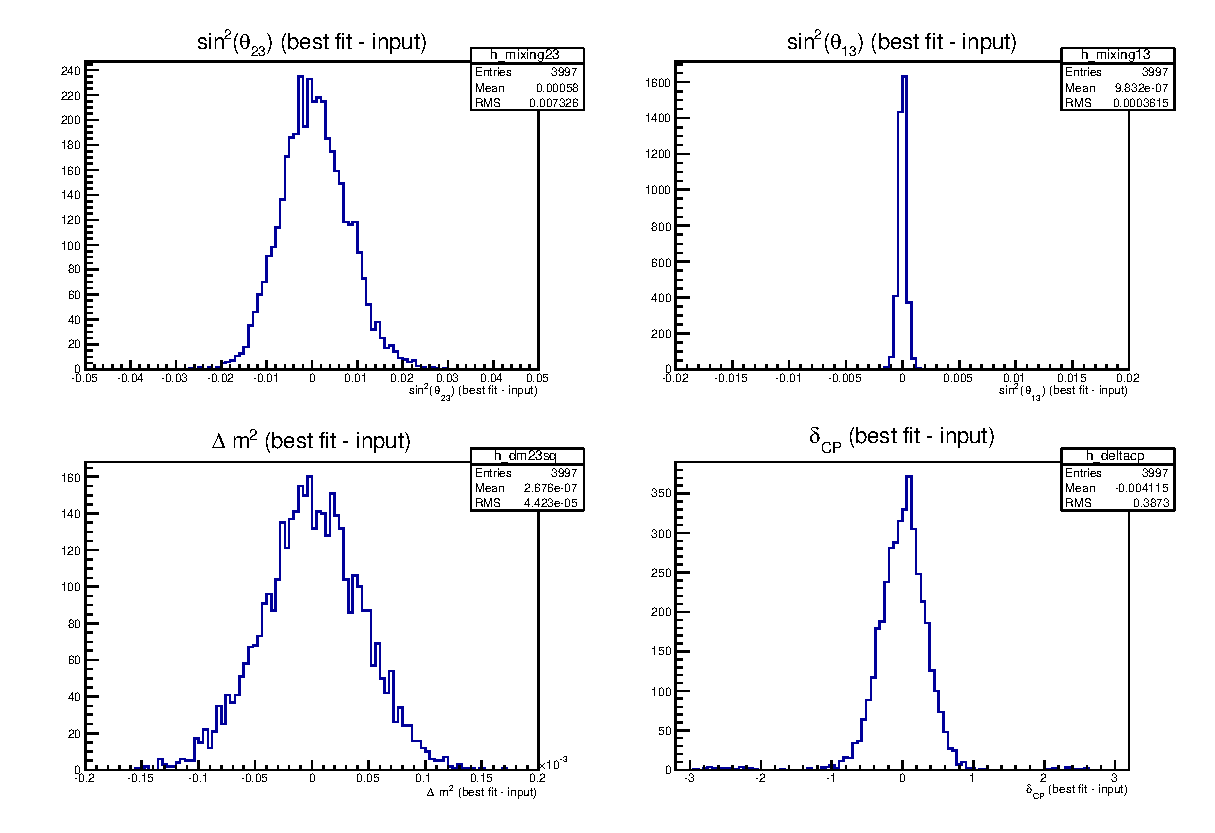
\includegraphics[width=0.7\textwidth]{images/appendix/deltacp/Dist_theta_minos_final_10const.eps}
\caption{Distribution of residuals of the four oscillation parameters in the '4 + 0' fit for oscillation point
with values $\sin^{2}\theta_{23}= 0.34$, $|\Delta m^{2}| = 2.4\times10^{-3}(eV^{2}/c^{4})$, $\sin^{2}\theta_{13}=0.025$ and $\delta_{CP} = 0$
at the T2K goal POT ($7.8\times 10^{21}$) constraining $\sin^{2}\theta_{13}$ with an error of 10\%.}
\label{fig:residualsfinalconstrainingtheta13}
\end{center}
\end{figure}

The sensitivity improves when constraining $\theta_{13}$ since $\delta_{CP}$ is always found in combination with $\sin \theta_{13}$ in the PMNS matrix:
\begin{equation}
U = \left( \begin{array}{ccc} 1 & 0 & 0 \\  0 & c_{23} & s_{23} \\ 0 & -s_{23} & c_{23}\\ \end{array} \right) \times \left( \begin{array}{ccc}  c_{13} & 0 & s_{13}e^{-i\delta} \\ 0 & 1 & 0 \\ - s_{13}e\
\
^{i\delta} & 0 & c_{13}\\ \end{array} \right) \times \left( \begin{array}{ccc}  c_{12} & s_{12} & 0 \\ -s_{12} & c_{12} & 0 \\ 0 & 0 & 1\\ \end{array} \right)
\label{eq:PMNS}
\end{equation}

The test presented in Fig. \ref{fig:residualsfinalconstrainingtheta13} shows that the distribution of residuals is well behaved and centered at the
true value also for $\delta_{CP}$ at larger POT, discarding any intrinsic problems in the fitter. It can be repeated for different true input values of 
$\delta_{CP}$. Figures \ref{fig:residualsfinalconstrainingtheta13halfpi} and \ref{fig:residualsfinalconstrainingtheta13mhalfpi} shows the same study of residuals for a true input value of 
$\delta_{CP} =  \pi/2$ and $\delta_{CP} =  -\pi/2$ respectively. The asymmetry in the residuals  for $\sin^{2}\theta_{13}$ in Figs. \ref{fig:residualsfinalconstrainingtheta13halfpi} and \ref{fig:residualsfinalconstrainingtheta13mhalfpi} can be explained with the shape of $P_{\nu_{\mu}\rightarrow \nu_{e}}$ in Fig. \ref{fig:oscprobdeltacp}. When the true input value is
$\delta_{CP} =  \pi/2$ then $P_{\nu_{\mu}\rightarrow \nu_{e}}$ is at a minimum, and any different value of $\delta_{CP}$ gives a larger $P_{\nu_{\mu}\rightarrow \nu_{e}}$ so that the fitter
tends to compensate this decreasing the fitted value of $\sin^{2}\theta_{13}$, creating a negative bias. The opposite happens when the true input value is
$\delta_{CP} = - \pi/2$: in this case $P_{\nu_{\mu}\rightarrow \nu_{e}}$ is at a maximum and any other value of $\delta_{CP}$ makes $P_{\nu_{\mu}\rightarrow \nu_{e}}$ to be smaller 
so that the fitter tries to compensate increasing the fitted value of $\sin^{2}\theta_{13}$, creating a positive bias.

\begin{figure}[htbp]
\begin{center}
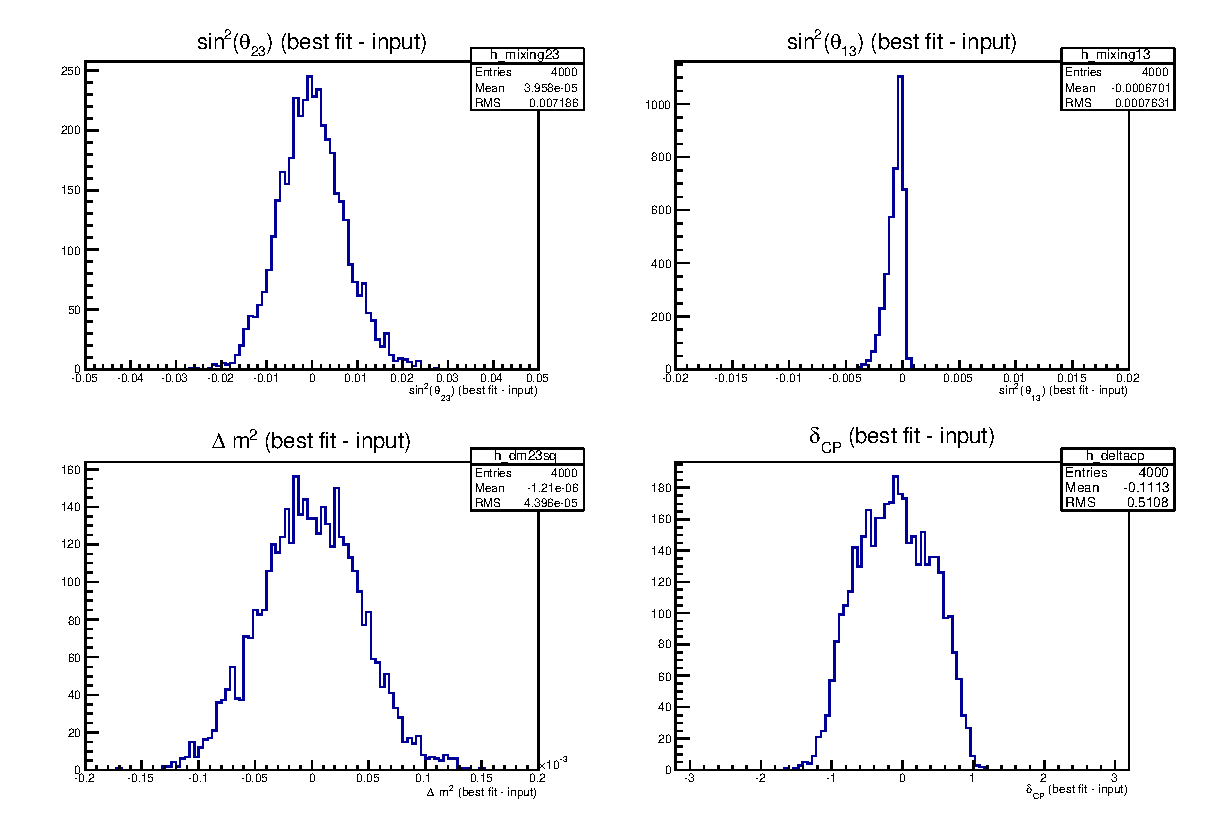
\includegraphics[width=0.7\textwidth]{images/appendix/deltacp/Dist_theta_minos_final_10const_pi2.eps}
\caption{Distribution of residuals of the four oscillation parameters in the '4 + 0' fit for oscillation point
with values $\sin^{2}\theta_{23}= 0.34$, $|\Delta m^{2}| = 2.4\times10^{-3}(eV^{2}/c^{4})$, $\sin^{2}\theta_{13}=0.025$
and $\delta_{CP} =  \pi/2$ at the T2K goal POT ($7.8\times 10^{21}$) constraining $\sin^{2}\theta_{13}$ with an error of 10\%.}
\label{fig:residualsfinalconstrainingtheta13halfpi}
\end{center}
\end{figure}


\begin{figure}[htbp]
\begin{center}
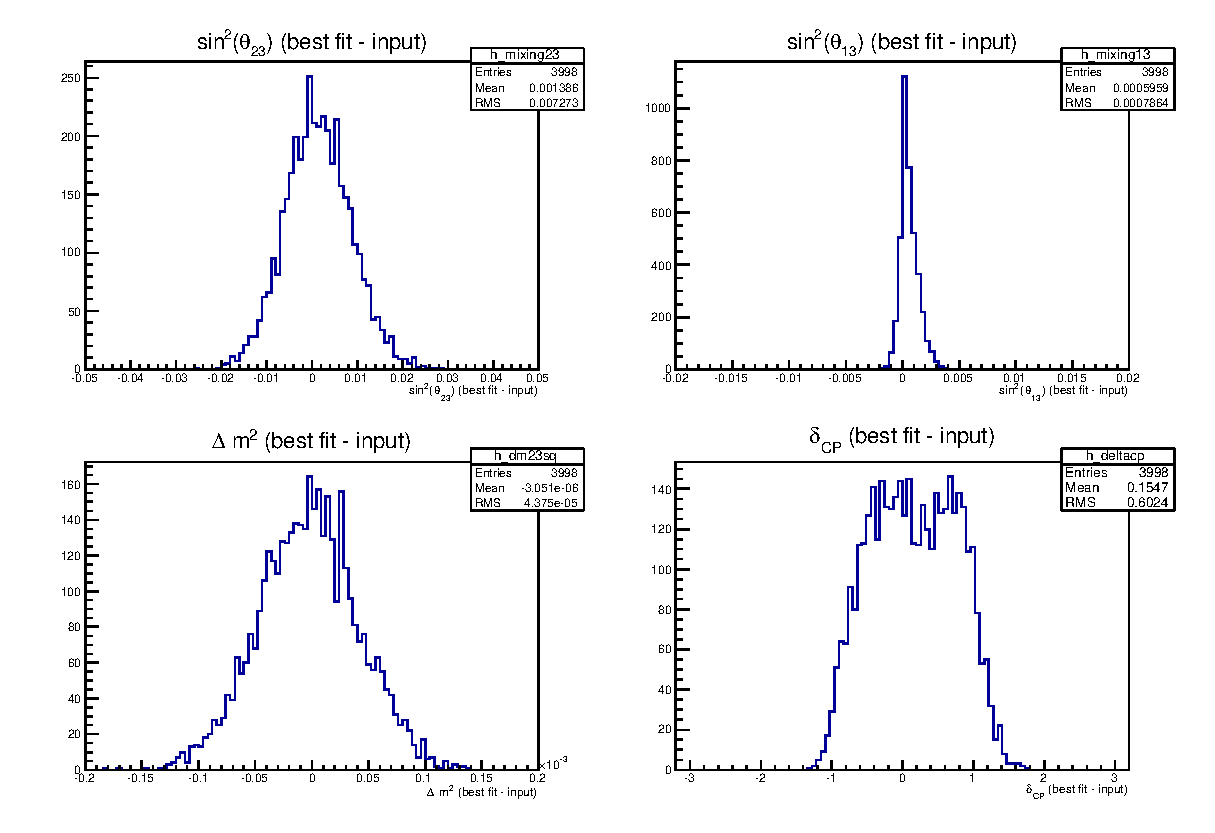
\includegraphics[width=0.7\textwidth]{images/appendix/deltacp/Dist_theta_minos_final_10const_mpi2.eps}
\caption{Distribution of residuals of the four oscillation parameters in the '4 + 0' fit for oscillation point
with values $\sin^{2}\theta_{23}= 0.34$, $|\Delta m^{2}| = 2.4\times10^{-3}(eV^{2}/c^{4})$, $\sin^{2}\theta_{13}=0.025$
and $\delta_{CP} =  -\pi/2$ at the T2K goal POT ($7.8\times 10^{21}$).}
\label{fig:residualsfinalconstrainingtheta13mhalfpi}
\end{center}
\end{figure}

From the results presented in this appendix it can be concluded that the distributions of residuals for $\delta_{CP}$ in figures \ref{fig:residuals_40_first}-\ref{fig:residuals_483_last} make sense. 


